\documentclass[tikz,border=10pt]{standalone}
\usetikzlibrary{shapes.geometric}

\begin{document}
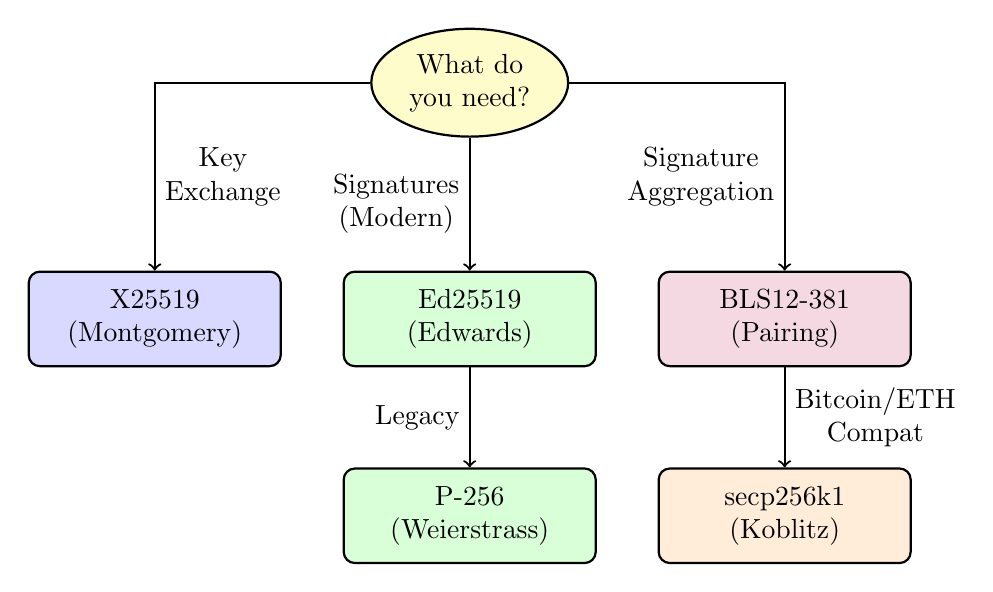
\begin{tikzpicture}[
  every node/.style={align=center},
  question/.style={ellipse, draw, thick, fill=yellow!20, minimum width=2.5cm, minimum height=1.2cm},
  answer/.style={rectangle, draw, thick, rounded corners, minimum width=3.2cm, minimum height=1.2cm}
]

% Central question
\node[question] (q) at (0,0) {What do\\you need?};

% Key Exchange
\node[answer, fill=blue!15] (x25519) at (-4,-3) {X25519\\(Montgomery)};

% Signatures - Modern
\node[answer, fill=green!15] (ed25519) at (0,-3) {Ed25519\\(Edwards)};

% Signatures - Legacy
\node[answer, fill=green!15] (p256) at (0,-5.5) {P-256\\(Weierstrass)};

% Aggregation
\node[answer, fill=purple!15] (bls) at (4,-3) {BLS12-381\\(Pairing)};

% Bitcoin/Ethereum
\node[answer, fill=orange!15] (secp) at (4,-5.5) {secp256k1\\(Koblitz)};

% Arrows with labels (orthogonal routing)
\draw[->, thick] (q) -| node[right, pos=0.75] {Key\\Exchange} (x25519);
\draw[->, thick] (q) -- node[left] {Signatures\\(Modern)} (ed25519);
\draw[->, thick] (ed25519) -- node[left] {Legacy} (p256);
\draw[->, thick] (q) -| node[left, pos=0.75] {Signature\\Aggregation} (bls);
\draw[->, thick] (bls) -- node[right] {Bitcoin/ETH\\Compat} (secp);

\end{tikzpicture}
\end{document}
